% !TeX TS-program = pdflatex
% !TeX encoding = UTF-8
% !TeX spellcheck = en_GB
% !TeX root = exam-main.tex
\documentclass[]{beamer}

\usepackage[T1]{fontenc}
\usepackage{textcomp}
\usepackage[utf8]{inputenc}
\usepackage{babel}

% ------------------ %
%% Presentation settings %%
\usepackage{appendixnumberbeamer}
%\mode<presentation>
\usetheme[progressbar=foot,numbering=counter]{metropolis}
%\useoutertheme[right]{sidebar}
\setbeamercovered{dynamic}
%\setbeamertemplate{blocks}[default]%[shadow=true]
\setbeamertemplate{sections/subsections in toc}[circle]
\setbeamertemplate{items}[circle]
\setbeamertemplate{navigation symbols}{}
\metroset{block=fill}

%\mode<all>
% ------------------ %
%% Floating objects %%
\graphicspath{{../r/plots/},{./Figures/}}
\usepackage{booktabs}
%\usepackage{caption}
%\captionsetup{format=hang,labelsep=colon}%,font={small,rm},labelfont={sf,bf}}
%\captionsetup[table]{skip=-0.9\medskipamount,position=top}
% ------------------ %
%% Mathematical stuffs %%
\usepackage{mathtools}
%\newcommand{\numberset}{\mathbb}
%\newcommand{\R}{\numberset{R}}
\DeclareMathOperator{\sign}{sign}
\DeclareMathOperator*{\argmin}{arg\,min}
\DeclareMathOperator*{\argmax}{arg\,max}
%\DeclarePairedDelimiter{\abs}{\lvert}{\rvert}
%\DeclarePairedDelimiter{\norm}{\lVert}{\rVert}
\DeclarePairedDelimiter{\set}{\{}{\}}
%\renewcommand{\epsilon}{\varepsilon}
\renewcommand{\phi}{\varphi}
%\theoremstyle{definition}
%\newtheorem{defs}{Definition}
%\theoremstyle{plain}
%\newtheorem{thm}{Theorem}
% ------------------ %
%% Drawings %%
\usepackage{pgfplots} % + tikz
\pgfplotsset{compat=newest}
\usetikzlibrary{shapes,calc}

\tikzstyle{treenode} = [draw,circle,minimum width=0.6cm,font=\footnotesize,text centered,
inner sep=1.5pt,outer sep=0pt]
\tikzstyle{cloud} = [draw,ellipse,centered,text width=3.5em,text centered,
inner sep=0.5pt,outer sep=0pt,fill=mLightBrown!20,font=\footnotesize]
\tikzstyle{cloud2} = [draw,ellipse,centered,text width=3.2em,text centered,
inner xsep=0pt,outer sep=0pt,fill=mLightBrown!20,font=\small]
\tikzstyle{cloud3} = [draw,ellipse,centered,text centered,text width=1cm,
inner ysep=5pt,inner xsep=0pt,outer sep=0pt,fill=mLightBrown!20,font=\small]
% ------------------ %
%% Code %%
% ------------------ %
%% Numbers %%
\usepackage{siunitx}
\sisetup{%
	output-decimal-marker={.},group-separator={\,},%
	%	round-mode=places,round-precision=6,%
	table-parse-only,table-number-alignment=center%
}
% ------------------------------- %
\usepackage{listings}
\definecolor{Rkwd}{rgb}{0.737,0.353,0.396}
\definecolor{Rparam}{rgb}{0.333,0.667,0.333}
\definecolor{Rnum}{rgb}{0.686,0.059,0.569}
\definecolor{Rstr}{rgb}{0.192,0.494,0.8}
\definecolor{Rcomm}{rgb}{0.678,0.584,0.686}
% R
\lstdefinestyle{Rlang}{language=R,%
	keywordstyle=\color{Rkwd},basicstyle=\small\ttfamily,%
	commentstyle=\color{Rcomm}\ttfamily\em,%
	stringstyle=\color{Rstr}\rmfamily,%
%	numbers=left,numberstyle=\tiny\color{green},stepnumber=1,numbersep=5pt,%
%	showstringspaces=false,breaklines=true,frameround=ftff,%
%	frame=lines,backgroundcolor=\color{lightergray},firstnumber=last,%
	deletekeywords={data,model},%
	morekeywords={TRUE,FALSE,NULL},%
	escapeinside={£!}{!£},%
}
\lstset{style=Rlang}
% ------------------ %
%% Pseudo-code %%
\usepackage[ruled,linesnumbered]{algorithm2e}
\SetNlSty{texttt}{}{}
\SetKw{Or}{or}
\SetKw{And}{and}
\SetKw{Not}{not}
% ------------------ %
%% Printing the presentation %%
%\usepackage{pgfpages}
%\pgfpagesuselayout{4 on 1}[a4paper,border shrink=5mm,landscape]
% ------------------ %
%% Presentation cover %%
%\title{Kinds of Gradient Boosting}
\title{Kinds of Ensembles}
\subtitle{Tested on \dots dataset}
\author{David Nardi}
\date{June 11, 2024}
\institute[UniFi]{MSc in AI, University of Florence}
%\logo{\includegraphics[width=0.2\textwidth]{./Figures/logo}}
%\titlegraphic{\includegraphics{./Figures/logo}}
% ------------------ %
%\usepackage{showframe}
\begin{document}

\pdfbookmark[1]{Title page}{cover}
\maketitle

% ------------------------------- %
% !TeX spellcheck = en_GB

% ------------------------------- %

\begin{frame}{Apple quality dataset}

\vspace*{-2.5em}\begin{columns}[T]
%\hspace*{2em}%
\begin{column}{0.5\textwidth}
Variables

%\begingroup\setlength{\tabcolsep}{0.25ex}
%\hspace*{-0.5em}\begin{tabular}{p{0.55\textwidth}p{0.5\textwidth}}
%\begin{itemize}
%	\item \texttt{Size}
%	\item \texttt{Weight}
%	\item \texttt{Sweetness}
%	\item \texttt{Crunchiness}
%\end{itemize}
%&
%\begin{itemize}
%	\item \texttt{Juiciness}
%	\item \texttt{Ripeness}
%	\item \texttt{Acidity}
%\end{itemize}
%\end{tabular}
%\endgroup

\begin{itemize}
	\item \texttt{Size}
	\item \texttt{Weight}
	\item \texttt{Sweetness}
	\item \texttt{Crunchiness}
	\item \texttt{Juiciness}
	\item \texttt{Ripeness}
	\item \texttt{Acidity}
\end{itemize}

\end{column}
\hspace*{-2em}%
\begin{column}{0.5\textwidth}
\alert{Binary classification} task% $\mathcal{Y}\in\set{0,1}$% (disease -- no disease)

Class distribution: 0.49 -- 0.51

\vspace{1em}Methods
\begin{itemize}
	\item $k\text{NN}$, Decision tree, Logistic regression
	\item Random forest
	\item AdaBoost
	\item Super learner
\end{itemize}
\end{column}
\end{columns}

\end{frame}


%- **Size**: size of the apple
%- **Weight**: weight of the apple
%- **Sweetness**: how sweet an apple is (Grado di dolcezza del frutto (concentrazione di zuccheri))
%- **Crunchiness**: how crisp the apple is (Croccantezza sulla base della consistenza del frutto)
%- **Juiciness**: how juicy an apple is (Succosità)
%- **Ripeness**: how ripe an apple is (Stato di deperibilità del frutto, quanto è maturo)
%- **Acidity**: how acid an apple is (Acidità (contenuto e composizione di acidi organici))
%- **Quality**: the quality is *good* or *bad*

% ------------------------------- %

\begin{frame}[fragile]{Random forest}

\begin{columns}[T]
\begin{column}{0.65\textwidth}
\begin{figure}
\centering
\vspace*{-0.5em}\begin{tikzpicture}
	%draw,ellipse,fill=red!20,minimum height=2em,text centered,font=\sffamily\small
	\tikzset{help lines/.append style=pink}
%	\draw [help lines] (-1,-4) grid (7,2); \node[draw,circle,fill=red] at (0,0) {};
	
	\node[cloud3] (b1) at (0,0) {$\pi_1, m_1$};
	\node[cloud3] (b2) at ($(b1)+(1.8,0)$) {$\pi_2, m_2$};
	\node[cloud3] (B) at ($(b2)+(3,0)$) {$\pi_B, m_B$};
	\draw[-,dotted,very thick] (b1) to (b2);
	\draw[-,dotted,very thick] (b2) to (B);
	
	\node[] (T1) at ($(b1)+(0,-1.3)$) {$T_1$};
	\node[] (T2) at ($(b2)+(0,-1.3)$) {$T_2$};
	\node[] (TB) at ($(B)+(0,-1.3)$) {$T_B$};
	\draw[-stealth] ($(b1.south)+(0,-0.15)$) to (T1);
	\draw[-stealth] ($(b2.south)+(0,-0.15)$) to (T2);
	\draw[-stealth] ($(B.south)+(0,-0.15)$) to (TB);
	
	\begingroup\linespread{0.9}
	\node[font=\footnotesize,text width=4em,centered,text centered,inner sep=0pt] (m) at (3.3,0.7) {random predictors};
	\node[font=\footnotesize,text width=4em,centered,text centered,inner sep=0pt] (pi) at (3.1,-1.2) {random subsample};
	\endgroup
	\draw[-stealth] (m) to ($(b2.east)+(-0.2,0.1)$);
	\draw[-stealth] (pi) to ($(b2.south)+(-0.1,0.25)$);
	
	\node[rectangle,fill=mLightGreen!20,font=\large,right] (G) at (-0.8,-3) {$G(x)=\argmax_k\sum_{b=1}^B\mathbb{I}(T_b(x)=k)$};
	\node[rectangle,fill=red!20,font=\large,right] (mtry) at ($(G.west)+(0,-1)$) {$\mathtt{mtry}=\lfloor\sqrt{p}\rfloor$};
\end{tikzpicture}
\end{figure}
\end{column}
\begin{column}{0.45\textwidth}
\begin{lstlisting}
randomForest(x, y,
  importance=TRUE,
  ntree=500,
  ntree=B.oob£!$\,\alert{\leftarrow}B^\ast$!£)
\end{lstlisting}

\hspace*{-0.8em}\includegraphics[width=1.1\columnwidth]{../r-StatsLearn-Exam/src/plots/biasvar-rf-apple}

\end{column}
\end{columns}

\end{frame}

\begin{frame}{Random forest tuning}

\begin{columns}[T]
\hspace*{-3em}\begin{column}{0.5\textwidth}
	\includegraphics[width=1.23\columnwidth]{biasvar-rf-apple}
\end{column}
\hspace*{-2em}\begin{column}{0.5\textwidth}
	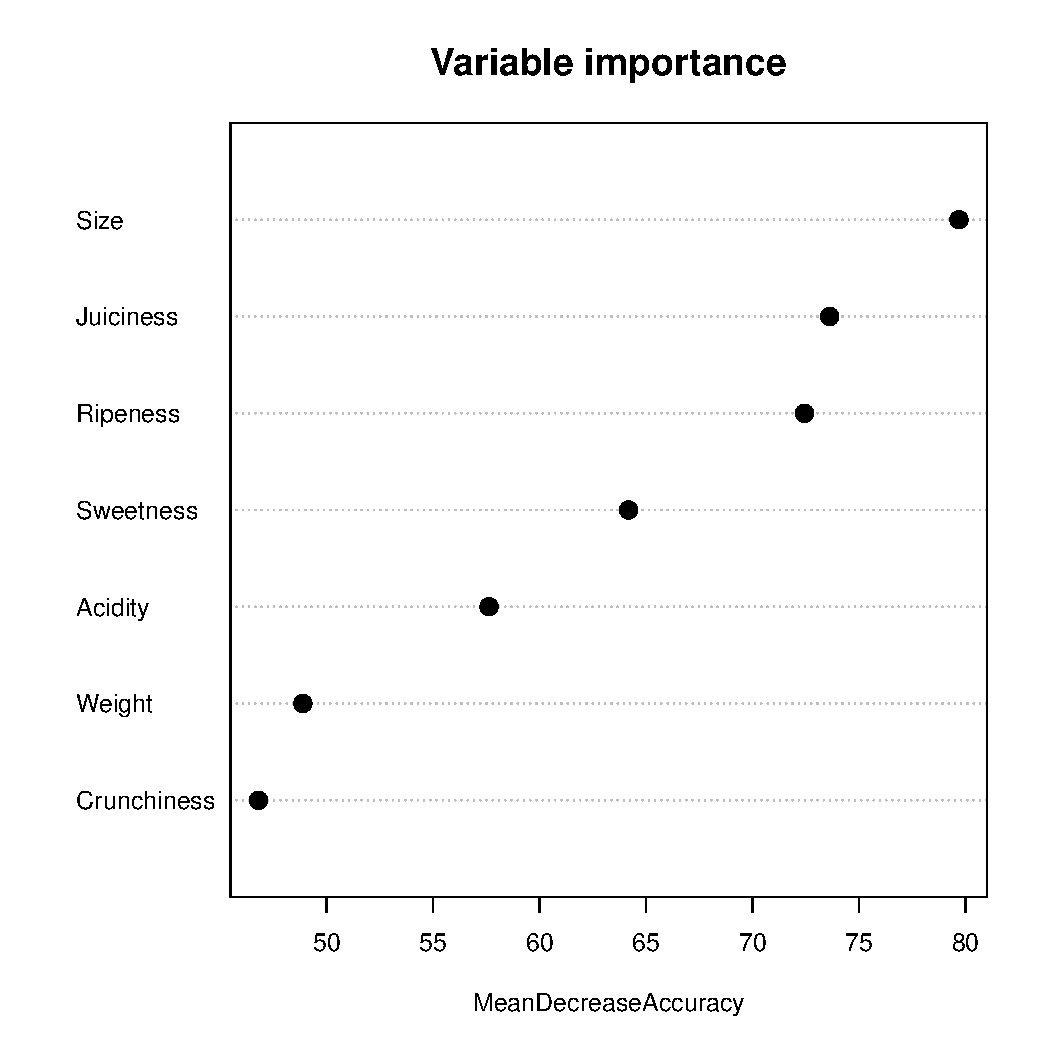
\includegraphics[width=1.23\columnwidth]{vip-rf-apple}
\end{column}
\end{columns}

\end{frame}

% ------------------------------- %

\begin{frame}[fragile]{AdaBoost algorithm}
% modello additivo perché in ogni albero c'è soltanto una variabile
\begin{columns}[T]
\begin{column}{0.48\textwidth}
\begin{figure}
\centering
\vspace*{-0.8em}\begin{tikzpicture}
	%draw,ellipse,fill=red!20,minimum height=2em,text centered,font=\sffamily\small
	\tikzset{help lines/.append style=pink}
%	\draw [help lines] (-2,-8) grid (3,1); \node[draw,circle,fill=red] at (0,0) {};
	
	\node[cloud2] (m1) at (0,0) {$w^{(1)}, \pi_1$};
	\node[cloud2] (m2) at (0,-1.25) {$w^{(2)}, \pi_2$};
	\node[cloud2] (M) at (0,-4.5) {$w^{(M)}, \pi_M$};
	\draw[-latex] (m1) to (m2);
	\draw[-,dotted,very thick] ($(m2.south) + (0,-0.15)$) to ($(M.north) + (0,+0.15)$);
	
	\node[right] (G1) at ($(m1)+(1.5,0)$) {$G_1, f_1, \alpha_1$};
	\node[right] (G2) at ($(m2)+(1.5,0)$) {$G_2, f_2, \alpha_2$};
	\node[right] (GM) at ($(M)+(1.5,0)$) {$G_M, f_M, \alpha_M$};
	\draw[-stealth] ($(m1.east) + (0.15,0)$) to (G1);
	\draw[-stealth] ($(m2.east) + (0.15,0)$) to (G2);
	%	\draw[-,dotted] (G2) to (GM);
	\draw[-stealth] ($(M.east) + (0.15,0)$) to (GM);
	
	%	\node[rectangle,fill=pink!80] (G) at (1.5,-6) {$G(x)=\sign\Bigl(\sum_{m=1}^M\beta_mG_m(x)\Bigr)$};
	\node[rectangle,fill=teal!20,font=\large,right] (G) at (-1,-5.55) {$f_m(x)=f_{m-1}(x)+\lambda\alpha_mG_m(x)$};
	\node[rectangle,fill=mLightGreen!20,font=\large,right] (L) at ($(G.west)+(0,-0.75)$) {$G(x)=\sign(f_M(x))$};
	\node[rectangle,fill=red!20,font=\large,right] (f) at ($(L.west)+(0,-0.75)$) {$L(y,f(x))=\exp(-yf(x))$};
	%	\draw[-stealth] (GM) to (G);
	
	\begingroup\linespread{0.9}
	\node[font=\footnotesize,text width=4em,centered,text centered,inner sep=0pt] (pi) at (2.8,-2.3) {random subsample};
	\node[font=\footnotesize,text width=4em,centered,text centered,inner sep=0pt] (w) at (1.1,-2.7) {sample weights};
	\endgroup
	\draw[-stealth] (pi) to ($(m2.east)+(-0.25,-0.1)$);
	\draw[-stealth] (w) to ($(m2.south)+(-0.25,0.25)$);
\end{tikzpicture}
\end{figure}
\end{column}
\begin{column}{0.48\textwidth}
%\vspace{0.7em}
%Journey to the final classifier:
%{\footnotesize\begin{itemize}
%\setlength{\itemsep}{-0.8ex}
%\item Linear combination of \alert{weak learners} (additive model)
%\item Adaptively build up complexity, through a prediction function
%\item Regularization with early stopping and shrinkage
%\item \alert{Re-weighting} of a bootstrapped fraction of the training data  % permette all'algoritmo di concentrarsi sugli esempi più difficili da classificare, quindi di questi esempi viene aumentato il peso
%\end{itemize}}

\vspace*{0.5em}Encoding $\mathcal{Y}\in\set{-1,1}$

\begin{lstlisting}
ada::ada(x, y,
  loss="exponential",
  type="discrete",
  iter£!$\,\alert{\leftarrow} M^\ast$!£, nu£!$\,\alert{\leftarrow}\lambda^\ast$!£,
  bag.frac£!$\,\alert{\leftarrow}\pi^\ast$!£,
  control=base.learner)
\end{lstlisting}

%\begin{columns}[T]
%\begin{column}{0.5\textwidth}
%\begin{tikzpicture}[]
%	\tikzset{help lines/.append style=pink}
%	%	\draw [help lines] (-2,-2) grid (2,1);
%	
%	\node[treenode] (root) at (0,0) {$-1$};
%	\node[treenode] (root-l) at (-120:1.35) {$-1$};
%	\node[treenode] (root-r) at (-60:1.35) {$1$};
%	
%	\draw[-] (root) -- node[font=\footnotesize,left] {$x_j<v$} (root-l);
%	\draw[-] (root) -- node[font=\footnotesize,right] {$x_j\geq v$} (root-r);
%\end{tikzpicture}
%\end{column}
%\hspace{-3em}\begin{column}{0.5\textwidth}
%\begin{tikzpicture}[]
%	\tikzset{help lines/.append style=pink}
%	%	\draw [help lines] (-3,-4) grid (3,1);
%	
%	\node[treenode] (root) at (0,0) {$-1$};
%	\node[treenode] (root-l) at (-130:1.4) {$-1$};
%	\node[treenode] (root-r) at (-50:1.4) {$1$};
%	\node[treenode] (ll) at ($(root-l)+(-110:1.25)$) {$1$};
%	\node[treenode] (lr) at ($(root-l)+(-70:1.25)$) {$-1$};
%	\node[treenode] (rl) at ($(root-r)+(-110:1.25)$) {$1$};
%	\node[treenode] (rr) at ($(root-r)+(-70:1.25)$) {$-1$};
%	
%	\draw[-] (root) -- (root-l);
%	\draw[-] (root) -- (root-r);
%	\draw[-] (root-l) -- (ll); \draw[-] (root-l) -- (lr);
%	\draw[-] (root-r) -- (rl); \draw[-] (root-r) -- (rr);
%\end{tikzpicture}
%\end{column}
%\end{columns}

\vspace{1.5em}\begin{center}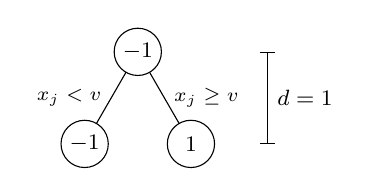
\begin{tikzpicture}[]
	\tikzset{help lines/.append style=pink}
%	\draw [help lines] (-2,-2) grid (2,1);
	
	\node[treenode] (root) at (0,0) {$-1$};
	\node[treenode] (root-l) at (-120:1.35) {$-1$};
	\node[treenode] (root-r) at (-60:1.35) {$1$};
	
	\draw[-] (root) -- node[font=\scriptsize,left] {$x_j<v$} (root-l);
	\draw[-] (root) -- node[font=\scriptsize,right] {$x_j\geq v$} (root-r);

	\draw[|-|] ($(root)+(1.65,0)$) -- node[right,font=\footnotesize] {$d=1$} ++ (0,-{1.35*cos(30)});
\end{tikzpicture}\end{center}

\end{column}
\end{columns}

\end{frame}

\begin{frame}{AdaBoost tuning}

% soltanto il CV error per questioni di spazio e comunque perché il training va diretto a 0 senza troppi complimenti

% per d>1 si perde la proprietà di additività del modello
% il vantaggio rispetto alla random forest lo perde un po'

\begin{columns}[T]
\hspace*{-2.4em}\begin{column}{0.5\textwidth}
	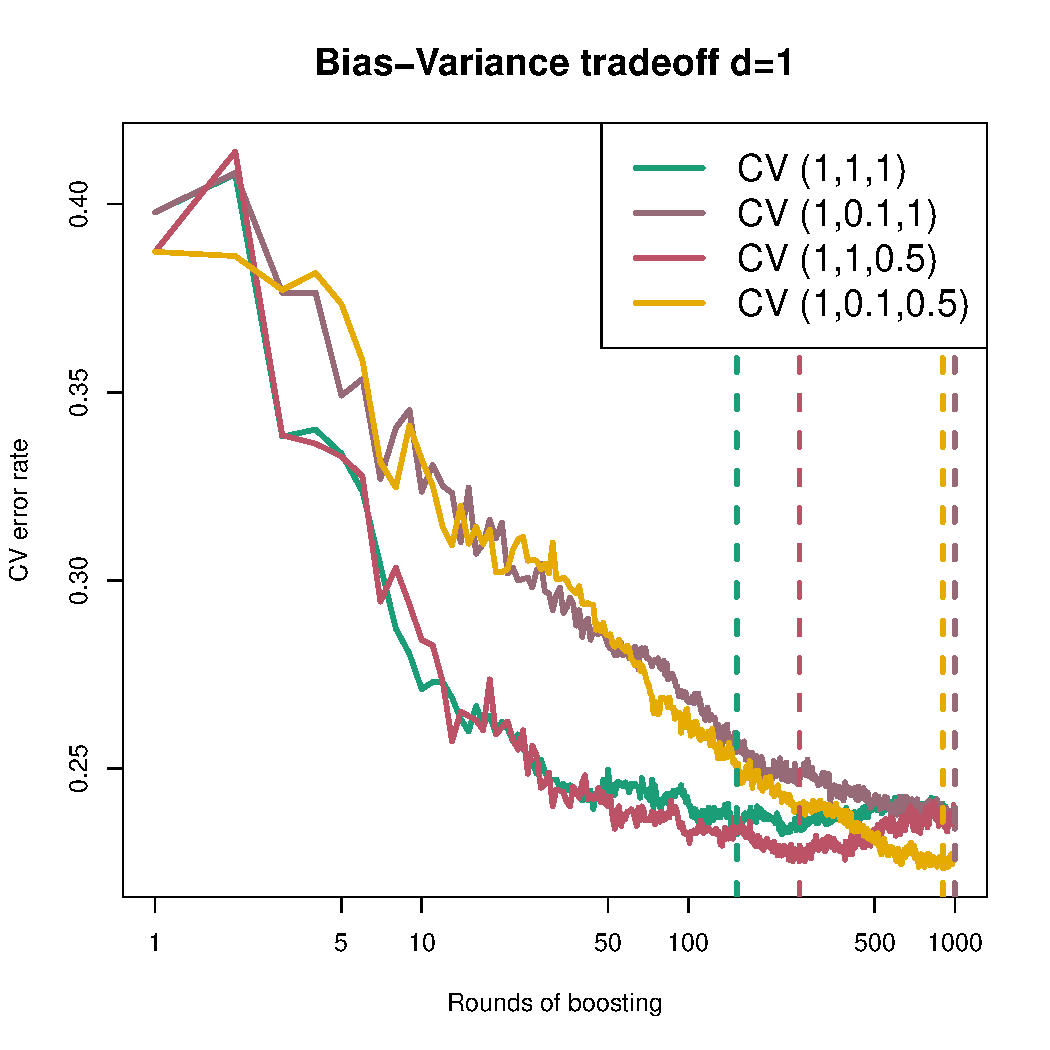
\includegraphics[width=1.23\columnwidth]{biasvar-ada1-apple}
	% oppure ci metto due parole sulla variable importance
\end{column}
\begin{column}{0.5\textwidth}
	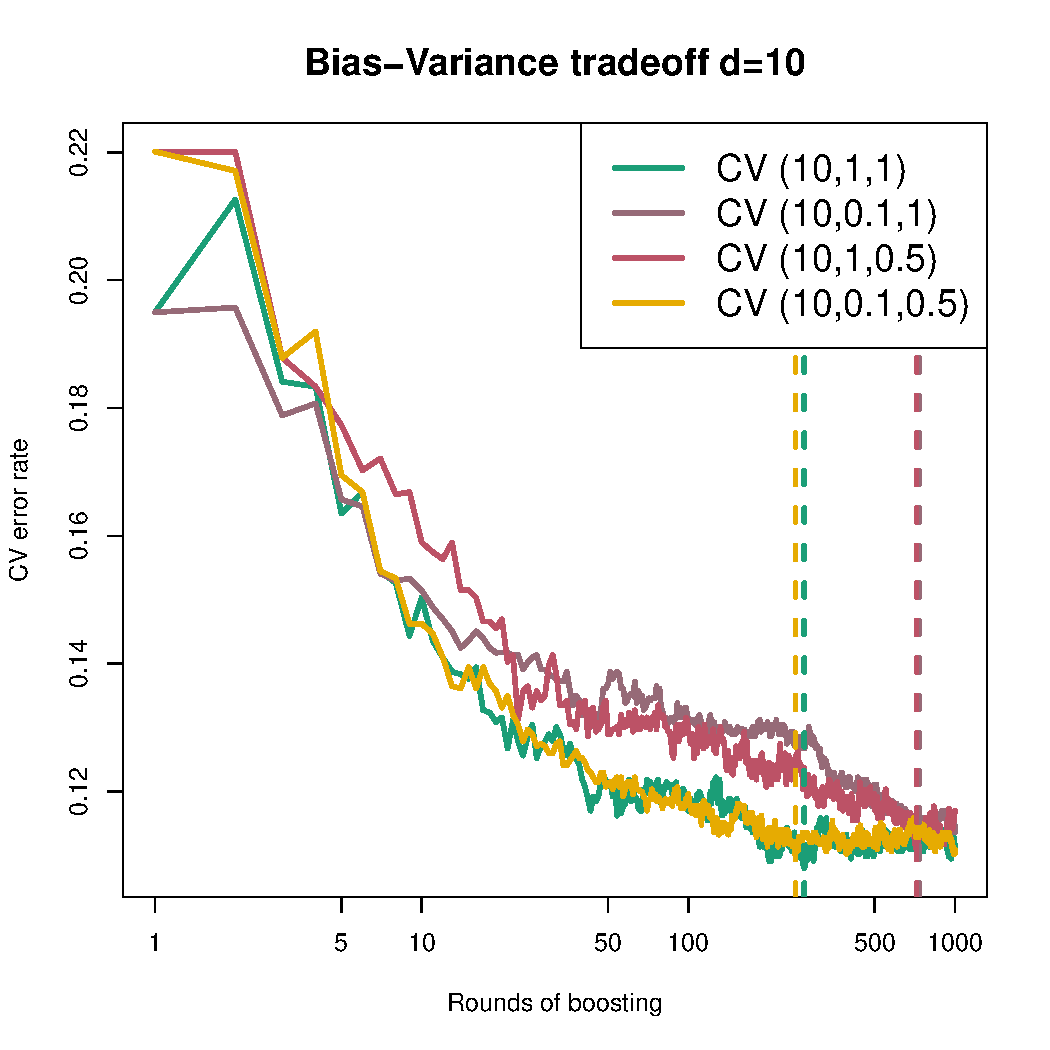
\includegraphics[width=1.23\columnwidth]{biasvar-ada2-apple}
\end{column}
\end{columns}

\end{frame}

% ------------------------------- %

\begin{frame}{AdaBoost variable importance}

% la scale sull'ascisse va bene?

% mi interessava riproporre questa analisi perché volevo indagare sulla differente selezione delle variabili da parte dei due modelli

\begin{columns}[T]
\hspace*{-3.5em}\begin{column}{0.5\textwidth}
	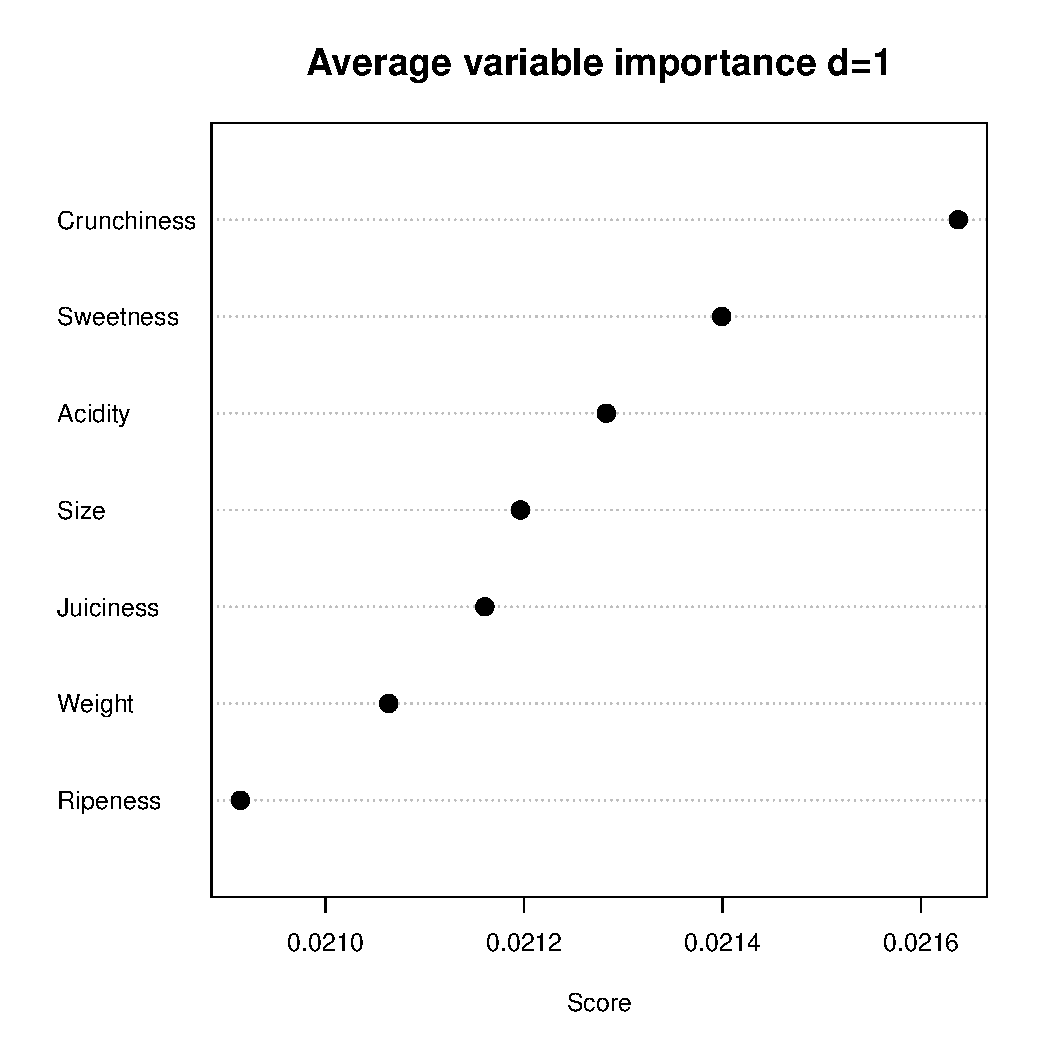
\includegraphics[width=1.23\columnwidth]{vip-ada1-apple}
\end{column}
\hspace*{-1.5em}\begin{column}{0.5\textwidth}
	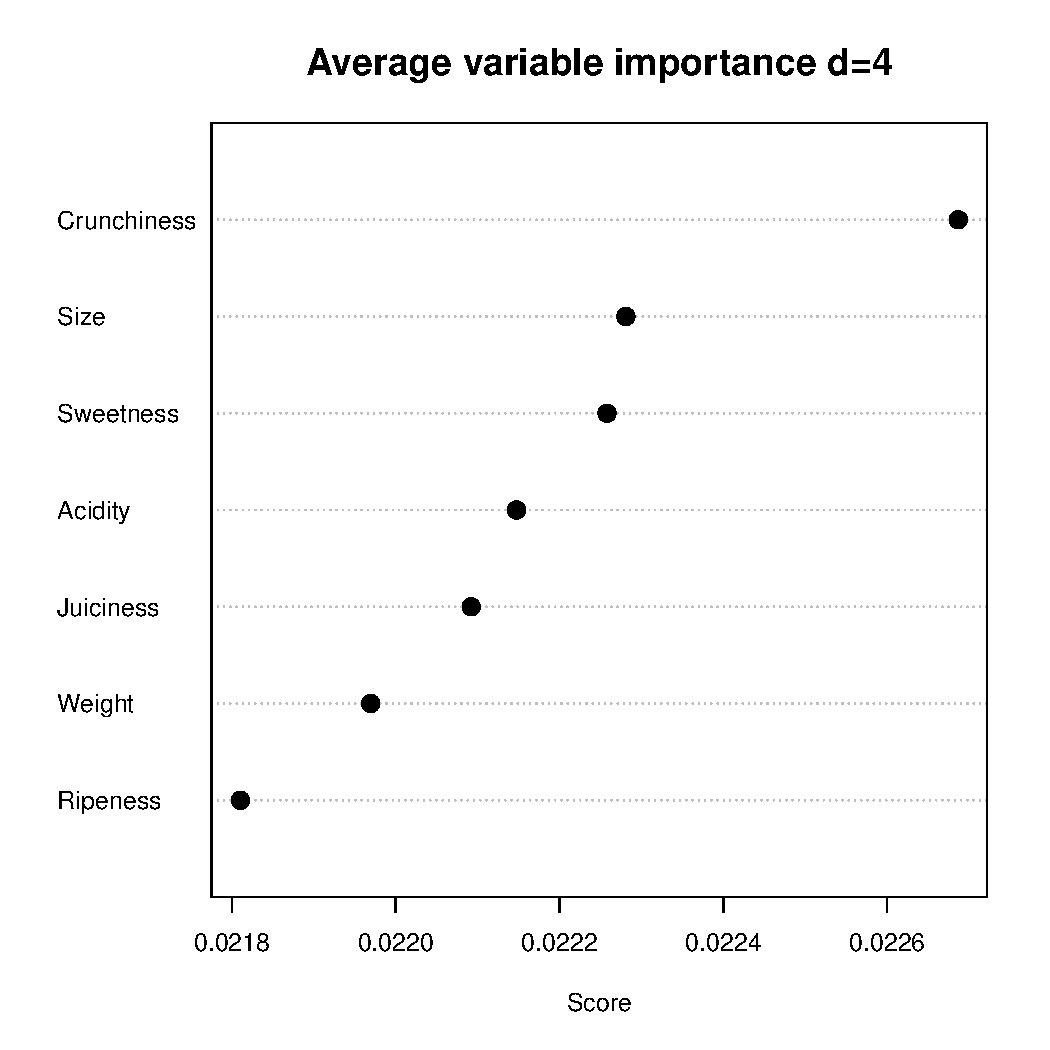
\includegraphics[width=1.23\columnwidth]{vip-ada2-apple}
\end{column}
\end{columns}

\end{frame}

% ------------------------------- %

\begin{frame}{Super Learner flow diagram}

\vspace*{0.25em}\begin{tikzpicture}
	\tikzset{help lines/.append style=pink}
%	\draw [help lines] (-5,-4) grid (6,4); \node[draw,circle,red] at (0,0) {};

	% start with full training data
	\node[right,font=\small] (data) at (-5,0) {$\mathcal{D}=\set{(x_i,y_i)}_1^N$};

	% path 1: full training data
	\node[draw,rectangle,minimum width=2cm,minimum height=0.5cm,font=\small] (full) at (-1,2) {$\hat{\phi}_1, \hat{\phi}_2,\dots,\hat{\phi}_K$};
	\begingroup\linespread{0.9}\node[font=\footnotesize,text centered,text width=2.5cm] at ($(full)+(0,0.8)$) {strong learners on full $\mathcal{D}$, $\hat{\phi}_k(\boldsymbol{X})$};\endgroup
	\begingroup\linespread{0.9}\draw[-latex,bend left,thick] (data.north) to node[font=\footnotesize,above left,text centered,text width=1.5cm] {learners prediction} (full.west);\endgroup

	% path 2: cross-validation for weights
	\node[font=\footnotesize,below] (cross) at (0,-1.5) {
		$\begin{array}{cccc|c}
			\hat{\phi}_1 & \hat{\phi}_2 &\dots & \hat{\phi}_K & Y \\
			1 & 1 & \dots & 1 & 1 \\
			2 & 2 & \dots & 2 & 2 \\
			\vdots & \vdots & \ddots & \vdots & \vdots \\
			V & V & \dots & V & V
		\end{array}$
	};
	\begingroup\linespread{0.95}\node[font=\footnotesize,text centered,text width=3cm] at ($(cross.north)+(0,0.4)$) {cross-validation $\hat{\phi}_{k,T(\nu)}(\boldsymbol{X}_{V(\nu)})$};\endgroup
	\begingroup\linespread{0.9}\draw[-latex,thick,bend right] (data.south) to node[font=\footnotesize,below left,text centered,text width=1.5cm] {prediction weights} (cross);\endgroup

	% end with prediction
	\node[left] (pred) at (6,0) {$\hat{\phi}_{\text{SL}}=\sum_{k=1}^K{\color{mLightGreen}\hat{\alpha}_k}{\color{mLightBrown}\hat{\phi}_k}$};
	\draw[-latex,bend left,thick,mLightBrown] (full.east) to (pred);
%	\draw[-latex,thick,bend right,mLightGreen] (cross) to node[font=\scriptsize,below right,mDarkTeal] {$\argmin_\alpha\sum_{i=1}^NL(Y_i,m(z_i\rvert\alpha))$} (pred);
	\draw[-latex,thick,bend right,mLightGreen] (cross) to (pred);
	\node[font=\scriptsize] (alph) at (4,3.3) {$\hat{\alpha}=\argmin_\alpha\sum_{i=1}^NL(Y_i,m(z_i\rvert\alpha))$};
	\node[font=\scriptsize] at ($(alph)+(0,-0.55)$) {$m(z\rvert\alpha)=\sum_{k=1}^K\alpha_k\hat{\phi}_{k,T(\nu)}\bigl(\boldsymbol{X}_{V(\nu)}\bigr)$};
\end{tikzpicture}

\end{frame}

\begin{frame}[fragile]{Super Learner in practice}

% esecuzione in parallelo specifica per Windows

% azzardo un po': i coefficienti del super learner potrebbero essere di aiuto nella scelta del modello definitivo

\begin{columns}[T]
\hspace*{-2em}\begin{column}{0.55\textwidth}
%\vspace*{1cm}%
\begin{lstlisting}
SuperLearner(Y, X,
  cluster,
  SL.library£!$\,\alert{\leftarrow}\set{\phi_k}$!£,
  cvControl=list(
    V=10,shuffle=FALSE))
\end{lstlisting}

\vspace{0.5em}What's in the ensemble?
\begin{itemize}
	\item Response variable mean $\bar{y}$
	\item Logistic Regression with $\alpha=\numlist{0;1;0.5}$
	\item Grown and pruned Decision Tree
	\item Random Forest
\end{itemize}
\end{column}
\hspace*{-3em}\begin{column}{0.5\textwidth}
% una sorta di variable importance ma per i pesi degli strong learners
\begin{tikzpicture}
%	\draw[help lines] (0,0) grid (6,6); \node[draw,circle,fill=red] at (0,0) {};
	\node[immagine] at (0,0) {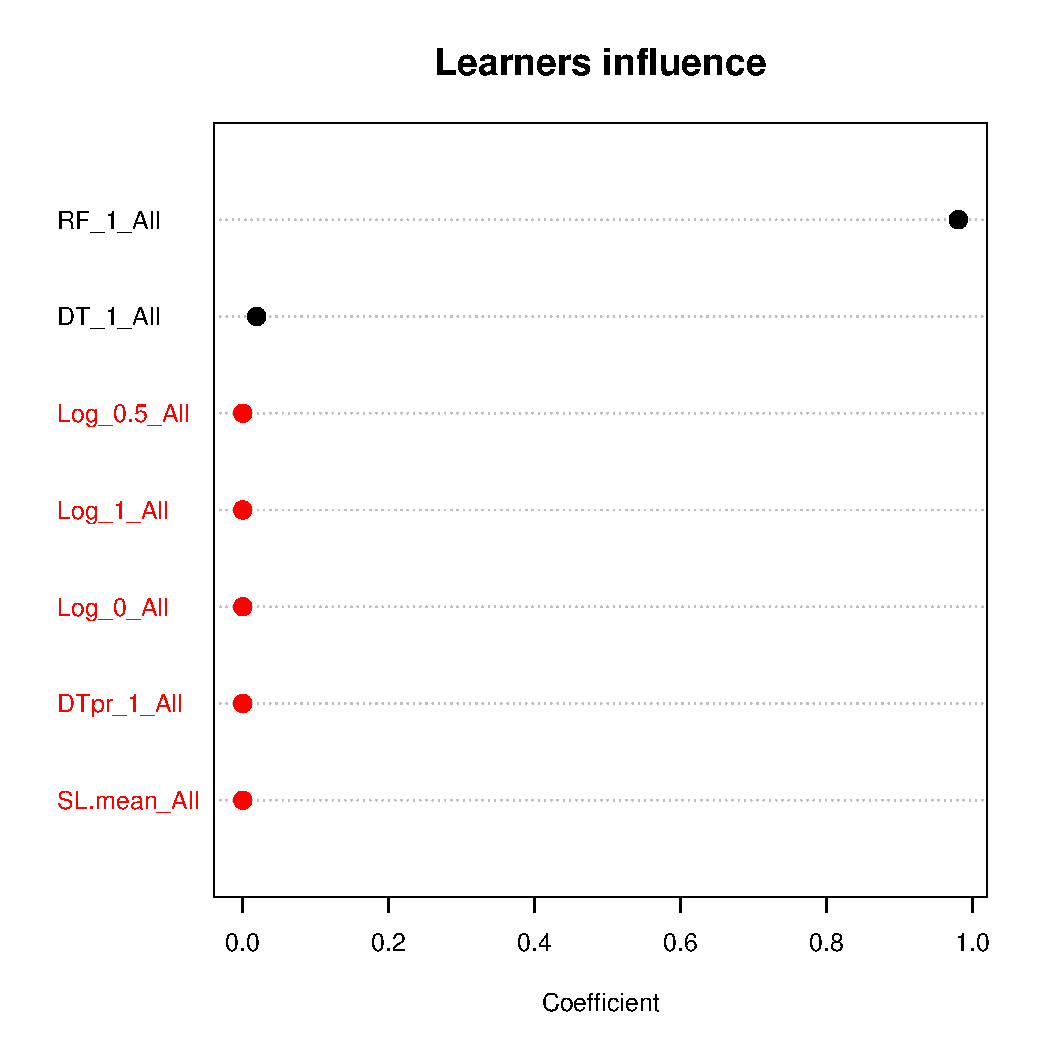
\includegraphics[width=1.23\columnwidth]{../r-StatsLearn-Exam/src/plots/coef-sl-apple}};

	\node[] (phi) at (0.7,6.4) {$\set{\hat{\phi}_k}$};
	\node[] (alph) at (2.25,0) {$\hat{\alpha}_k$};
	\draw[-latex,thick] (phi) -- ++(-90:0.8);
	\draw[-latex,thick] (alph) -- ++(13:1.1);
\end{tikzpicture}
%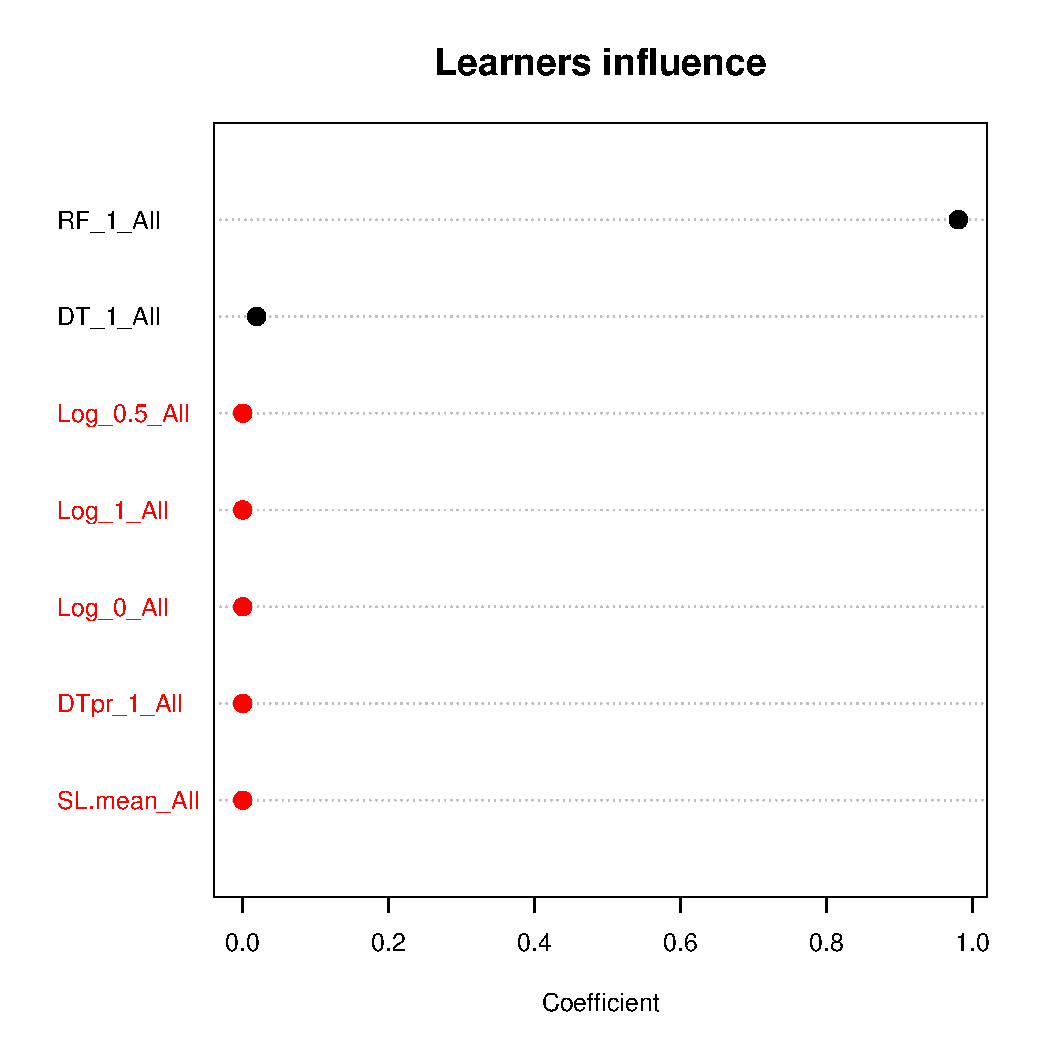
\includegraphics[width=1.23\columnwidth]{../r-StatsLearn-Exam/src/plots/coef-sl-apple}
\end{column}
\end{columns}

\end{frame}

% ------------------------------- %

\begin{frame}{Performance}

% il super learner riesce a prendere il meglio da questi modelli??

\begin{table}
\sisetup{round-mode=places}
\resizebox{0.9\textwidth}{!}{
\vspace*{-1em}\begin{tabular}{lS[round-precision=4]S[round-precision=4]}
\toprule
Model & {Train score} & {Test score} \\
\midrule
CART & 0. & 0. \\
Random forest & 0. & 0. \\
AdaBoost & 0. & 0. \\
Super learner & 0. & 0. \\
\bottomrule
\end{tabular}}
\end{table}

\end{frame}









% ------------------------------- %
%\appendix
%{\setbeamercolor{palette primary}{fg=black,bg=white}
%\begin{frame}[standout]
%%Thank you for your kindly attention!
%Questions?
%\end{frame}
%}
% ------------------------------- %
% !TeX spellcheck = en_GB

\appendix
\begin{frame}[allowframebreaks]{References}
\begin{thebibliography}{9}
	%% text book
	\bibitem{statslearn} T. Hastie, R. Tibshirani, and J. H. Friedman
	\newblock The Elements of Statistical Learning
	\newblock Springer, 2009.
	%% Super learner paper
	\bibitem{sup-learn} E. C. Polley, and M. J. van der Laan
	\newblock Super Learner in Prediction
	\newblock U.C. Berkeley Division of Biostatistics Working Paper Series. Working Paper 266, 2010
	%% AdaBoost package
	\bibitem{ada} M. Culp, K. Johnson and G. Michailidis
	\newblock \texttt{ada}: The R Package Ada for Stochastic Boosting
	\newblock Journal of Statistical Software, 17(2), 1–27, 2006
\end{thebibliography}
\end{frame}

% !TeX spellcheck = en_GB

\begin{frame}{$k\text{NN}$ and CART tuning}

\sideFigs{biasvar-knn-apple}{cp-tree-apple}

\end{frame}

% ------------------------------- %

%\begin{frame}[fragile]{Random forest}
%
%\begin{columns}[T]
%\begin{column}{0.7\textwidth}
%\begin{figure}
%\centering
%\hspace*{1em}\vspace*{-0.5em}%
%\begin{tikzpicture}
%	%draw,ellipse,fill=red!20,minimum height=2em,text centered,font=\sffamily\small
%	\tikzset{help lines/.append style=pink}
%	%	\draw [help lines] (-1,-4) grid (7,2); \node[draw,circle,fill=red] at (0,0) {};
%	
%	\node[cloud3] (b1) at (0,0) {$\pi_1, m_1$};
%	\node[cloud3] (b2) at ($(b1)+(1.8,0)$) {$\pi_2, m_2$};
%	\node[cloud3] (B) at ($(b2)+(3,0)$) {$\pi_B, m_B$};
%	\draw[-,dotted,very thick] (b1) to (b2);
%	\draw[-,dotted,very thick] (b2) to (B);
%	
%	\node[] (T1) at ($(b1)+(0,-1.3)$) {$T_1$};
%	\node[] (T2) at ($(b2)+(0,-1.3)$) {$T_2$};
%	\node[] (TB) at ($(B)+(0,-1.3)$) {$T_B$};
%	\draw[-stealth] ($(b1.south)+(0,-0.15)$) to (T1);
%	\draw[-stealth] ($(b2.south)+(0,-0.15)$) to (T2);
%	\draw[-stealth] ($(B.south)+(0,-0.15)$) to (TB);
%	
%	\begingroup\linespread{0.9}
%	\node[font=\footnotesize,text width=4em,centered,text centered,inner sep=0pt] (m) at (3.3,0.7) {random predictors};
%	\node[font=\footnotesize,text width=4em,centered,text centered,inner sep=0pt] (pi) at (3.1,-1.2) {random subsample};
%	\endgroup
%	\draw[-stealth] (m) to ($(b2.east)+(-0.2,0.1)$);
%	\draw[-stealth] (pi) to ($(b2.south)+(-0.1,0.25)$);
%	
%	\node[rectangle,fill=mLightGreen!20,font=\large,right] (G) at (-0.8,-3) {$G(x)=\argmax_k\sum_{b=1}^B\mathbb{I}(T_b(x)=k)$};
%	\node[rectangle,fill=red!20,font=\large,right] (mtry) at ($(G.west)+(0,-1)$) {$\mathtt{mtry}=\lfloor\sqrt{p}\rfloor$};
%\end{tikzpicture}
%\end{figure}
%\end{column}
%\hspace*{1em}\begin{column}{0.4\textwidth}
%\begin{lstlisting}
%randomForest(x, y,
%importance=TRUE,
%ntree=500,
%ntree=B.oob£!$\,\alert{\leftarrow}B^\ast$!£)
%\end{lstlisting}
%
%\vspace{1em}Loss-based variable importance
%
%%\hspace*{-0.8em}\includegraphics[width=1.1\columnwidth]{../r-StatsLearn-Exam/src/plots/biasvar-rf-apple}
%
%\end{column}
%\end{columns}
%
%\end{frame}

\begin{frame}{Random forest variable importance}

\begin{center}
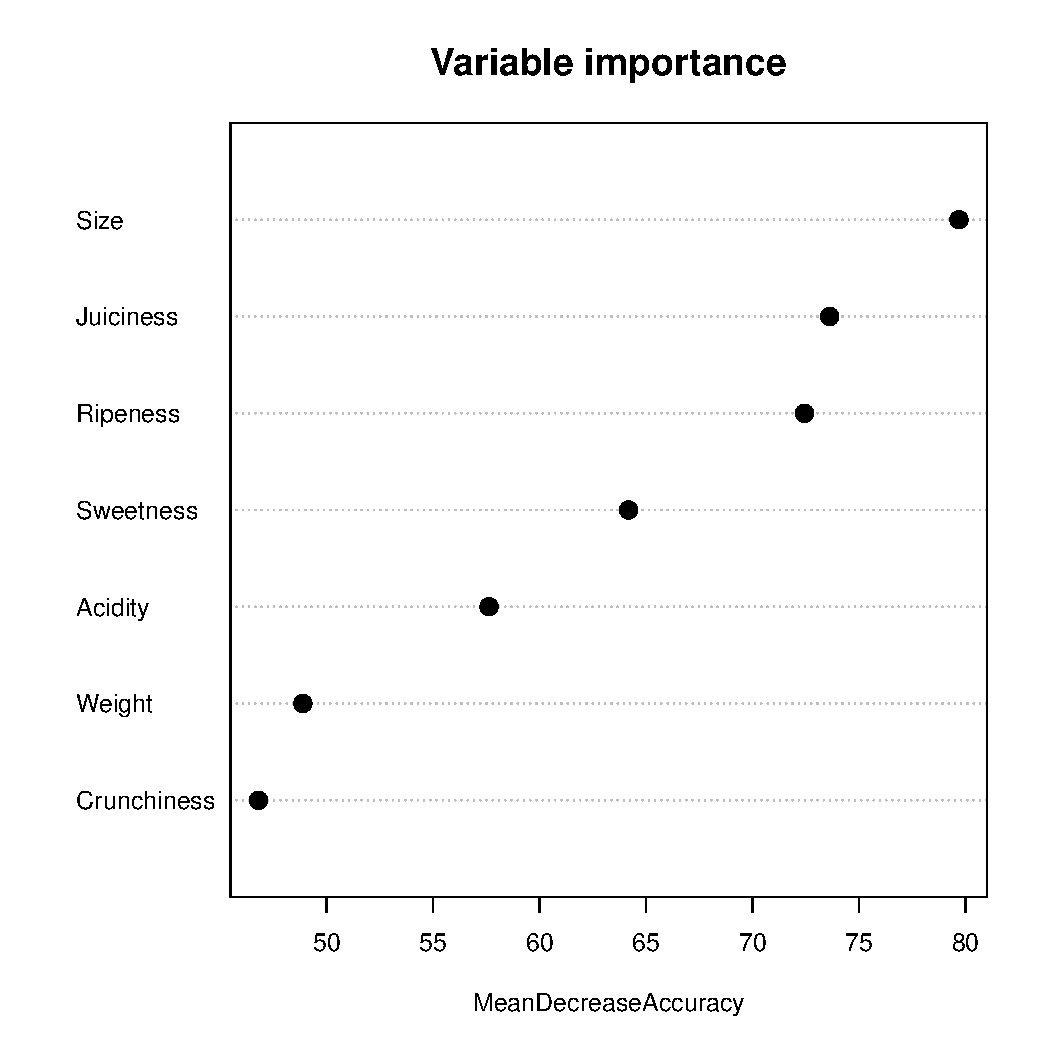
\includegraphics[width=0.7\textwidth]{vip-rf-apple}
\end{center}

\end{frame}

\begin{frame}{AdaBoost variable importance}

\begin{columns}[T]
\hspace*{-3.9em}%
\begin{column}{0.5\textwidth}
	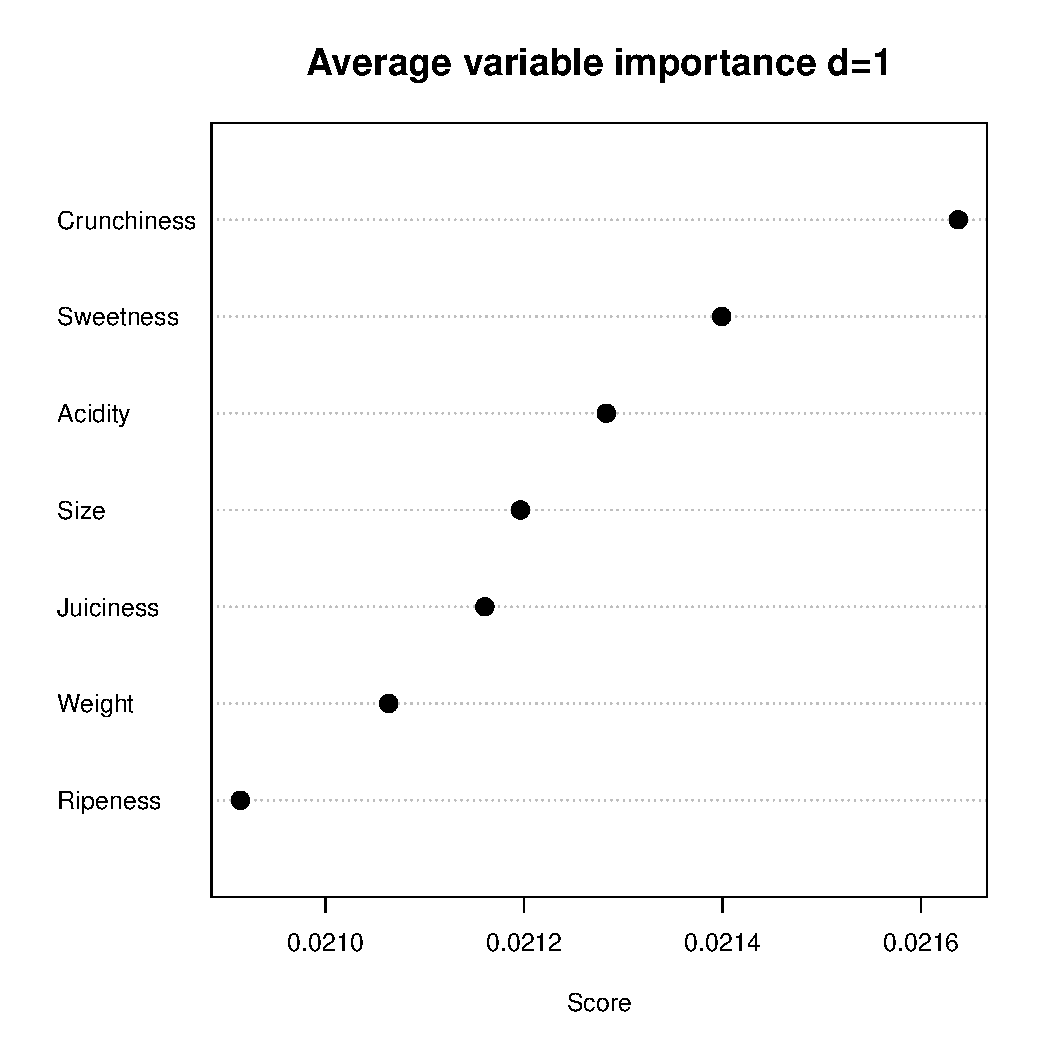
\includegraphics[width=1.25\columnwidth]{vip-ada1-apple}
\end{column}
\hspace*{-1em}%
\begin{column}{0.5\textwidth}
	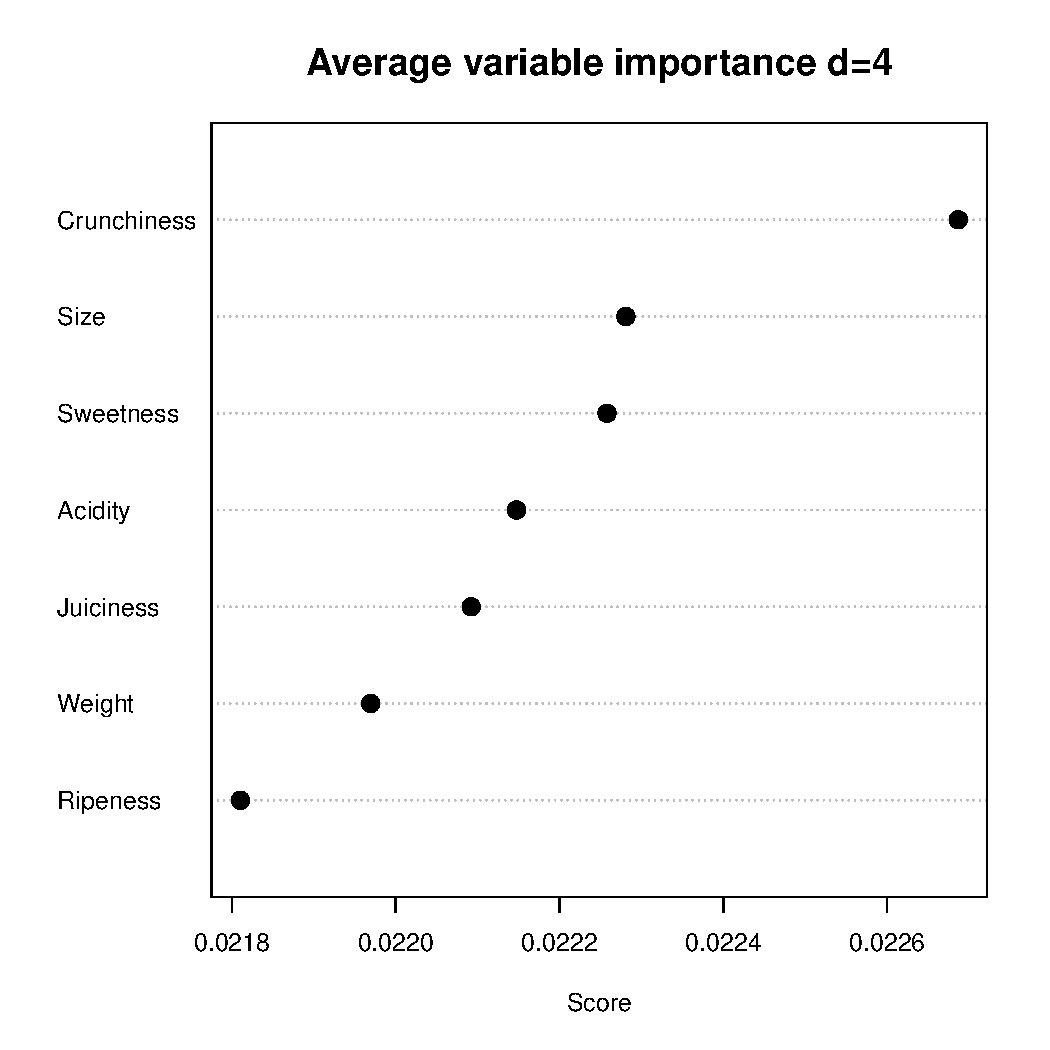
\includegraphics[width=1.25\columnwidth]{vip-ada2-apple}
\end{column}
\end{columns}

\end{frame}

% ------------------------------- %

\begin{frame}[fragile]{Discrete AdaBoost algorithm}
% stochastic setting
% stochastic gradient boosting framework, when bag.frac < 1
% -> shrinkage added
% -> out-of-bag fraction, on each iteration train a classifier on a different dataset sample, keep the rest as OOB

Discrete AdaBoost with shrinkage and out-of-bag, as an additive model with prediction function $f_m(x)$

{%
\setlength{\interspacetitleruled}{0pt}%
\setlength{\algotitleheightrule}{0pt}%
\begin{algorithm}[H]
\KwIn{$M$, $\set{(x_i,y_i)}_1^N$, $x_i\in\R^p$}
%Initialize observation weights $w_i^{(1)}=1/N$ s.t. $\sum_{i=1}^Nw_i^{(m)}=1$\;
Initialize $f_0(x)=0$\;
\For{$m=1$ \KwTo $M$}{
	Set $w_i^{(m)}=-\frac{\partial L(y,g)}{\partial g}\bigr\rvert_{g=f_m(x)}$ s.t.  $\sum_{i=1}^Nw_i^{(m)}=1$\;
	Fit classifier $G_m(x)$ using $w_i^{(m)}$ with samples from $\pi_m$\;
	Weighted error rate $\text{err}_m=\sum_{i=1}^Nw_i^{(m)}\mathbb{I}(y_i\neq G(x_i))$\;
	Set $\alpha_m=\frac{1}{2}\log\bigl(\frac{1-\text{err}_m}{\text{err}_m}\bigr)$\;
	Update $f_{m}(x)\gets f_{m-1}(x)+\lambda\alpha_mG_m(x)$\;
}
\KwOut{$G(x)=\sign(f_M(x))$}
\end{algorithm}}

\end{frame}

% ------------------------------- %

%\begin{frame}{Variable importance comparison}
%
%\begin{columns}[T]
%\hspace*{-4.2em}%
%\begin{column}{0.3\textwidth}
%	\begin{tikzpicture}
%		\tikzset{help lines/.append style=pink}
%%		\draw[help lines] (0,0) grid (5,5); \node[draw,circle,fill=red] at (0,0) {};
%		\node[immagine] (img) at (0,0) {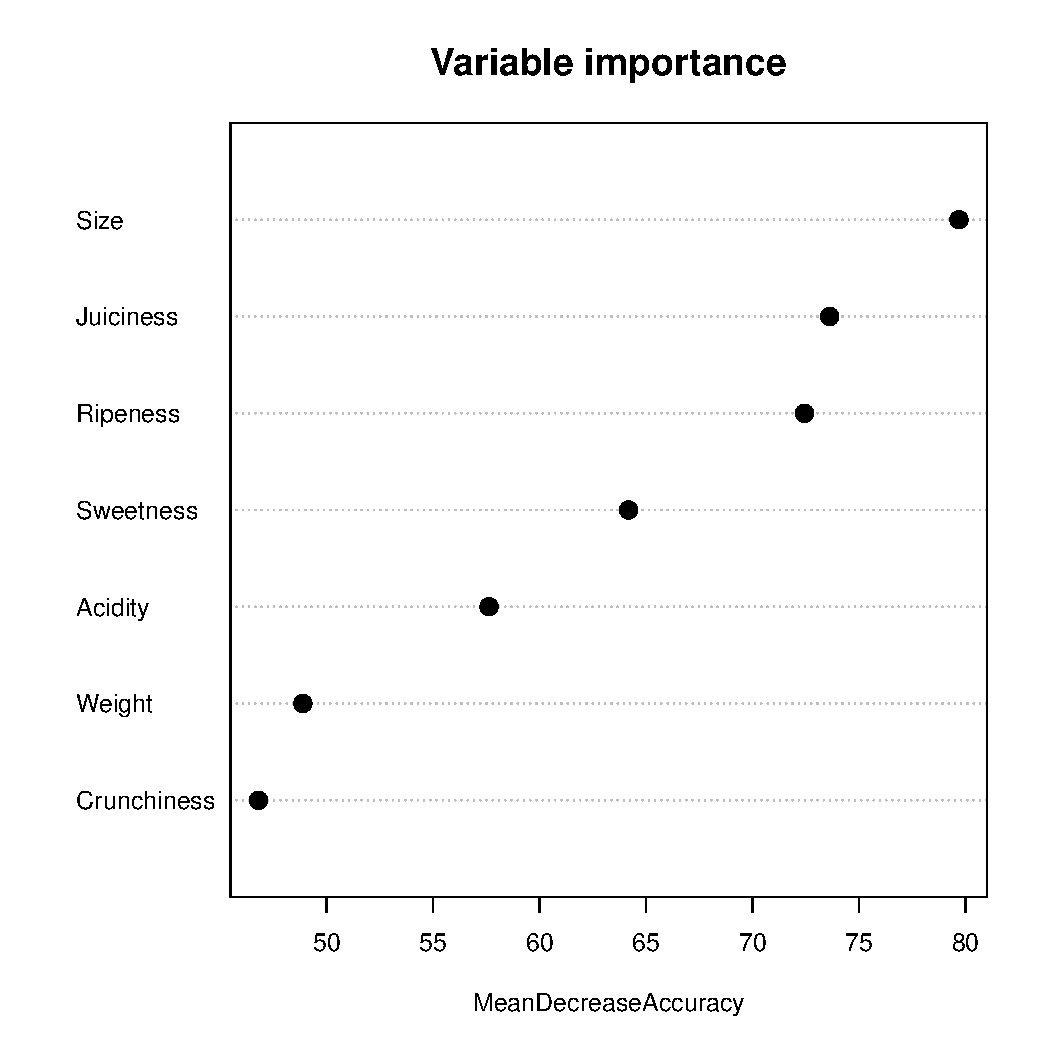
\includegraphics[width=1.475\columnwidth]{vip-rf-apple}};
%		\node[font=\small] at ($(img)+(0,2.8)$) {Random Forest};
%	\end{tikzpicture}
%\end{column}
%\hspace*{-0.7em}%
%\begin{column}{0.3\textwidth}
%	\begin{tikzpicture}
%		\node[immagine] at (0,0) {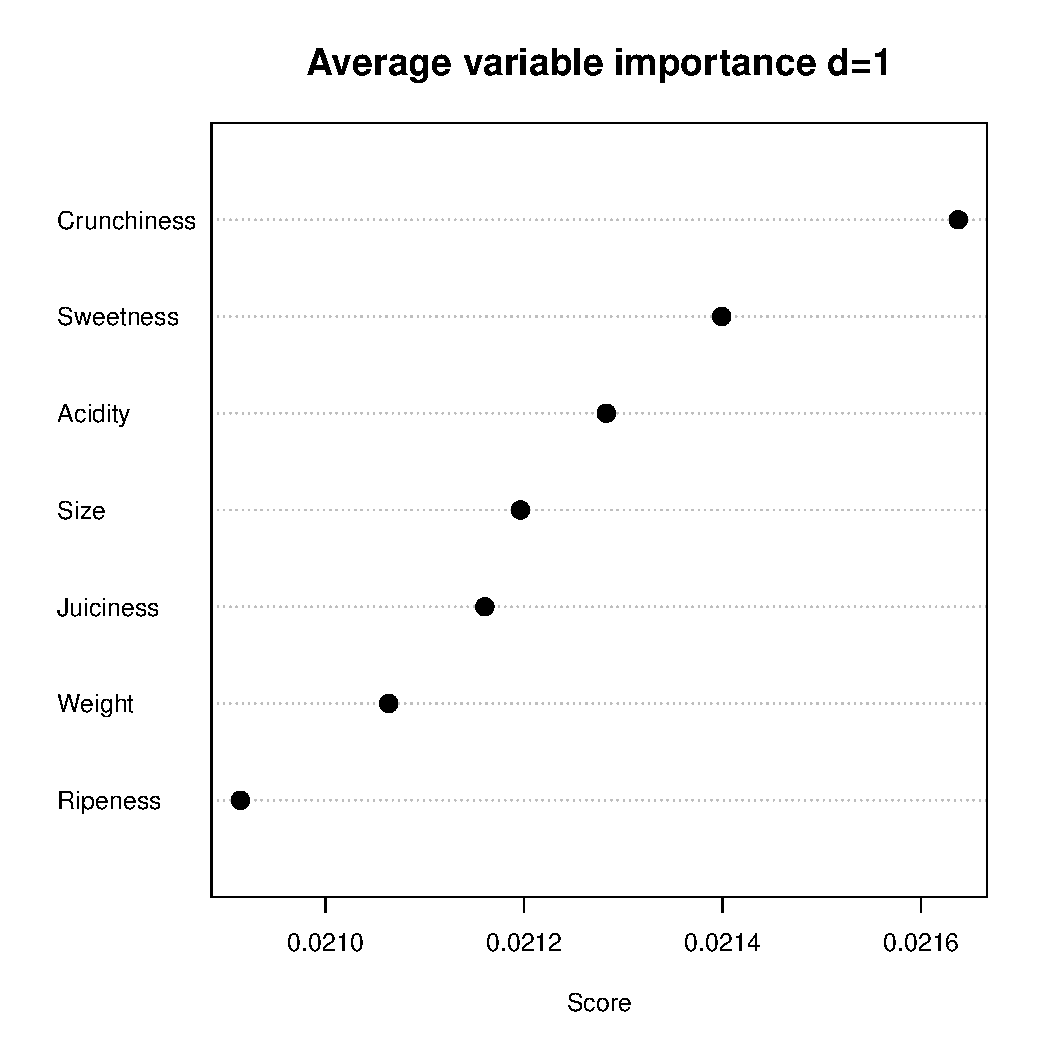
\includegraphics[width=1.475\columnwidth]{vip-ada1-apple}};
%		\node[font=\small] at ($(img)+(0,2.8)$) {$\text{AdaBoost}_{d=1}$};
%	\end{tikzpicture}
%\end{column}
%\hspace*{-0.7em}%
%\begin{column}{0.3\textwidth}
%	\begin{tikzpicture}
%		\node[immagine] at (0,0) {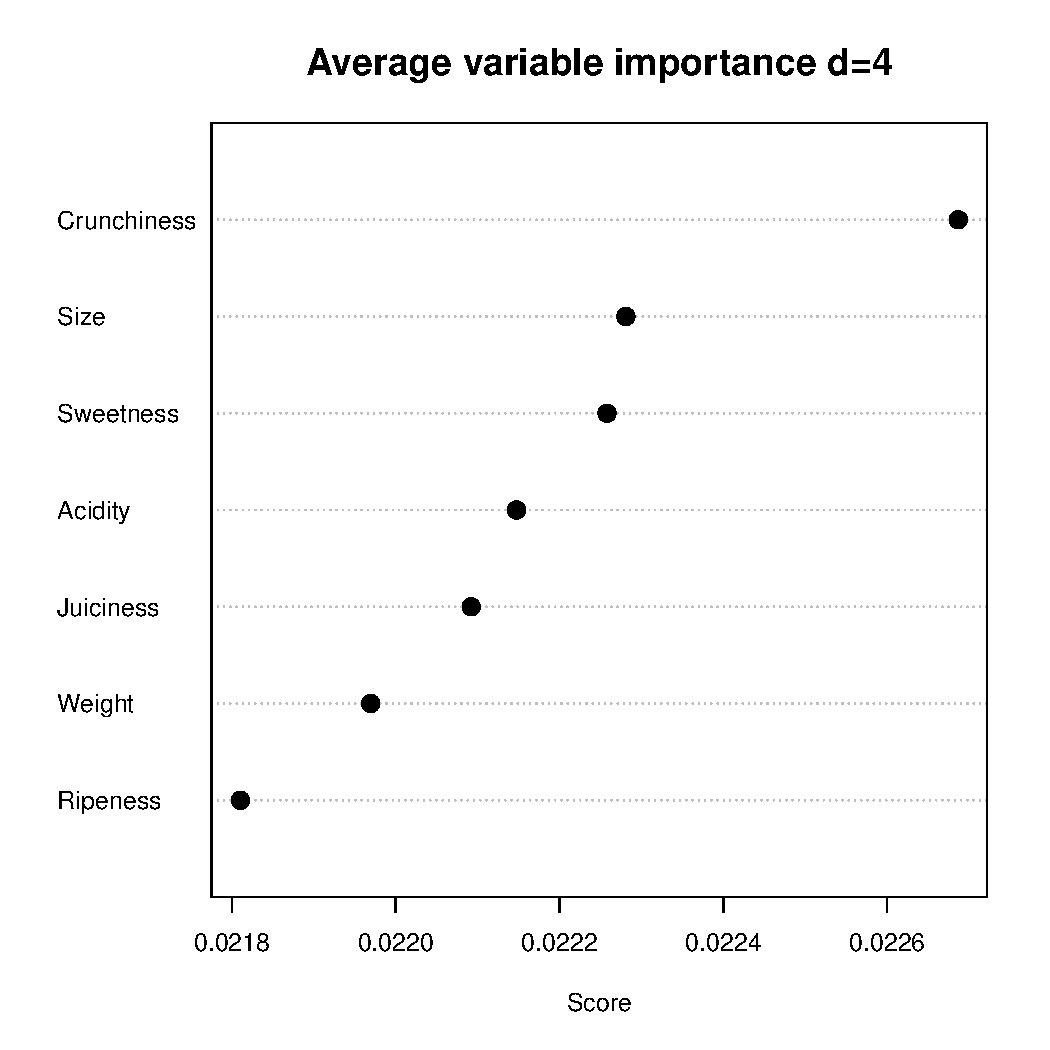
\includegraphics[width=1.475\columnwidth]{vip-ada2-apple}};
%		\node[font=\small] at ($(img)+(0,2.8)$) {$\text{AdaBoost}_{d=4}$};
%	\end{tikzpicture}
%\end{column}
%\end{columns}
%
%\end{frame}

% ------------------------------- %

\begin{frame}{Super Learner algorithm flow diagram}

\begin{figure}
	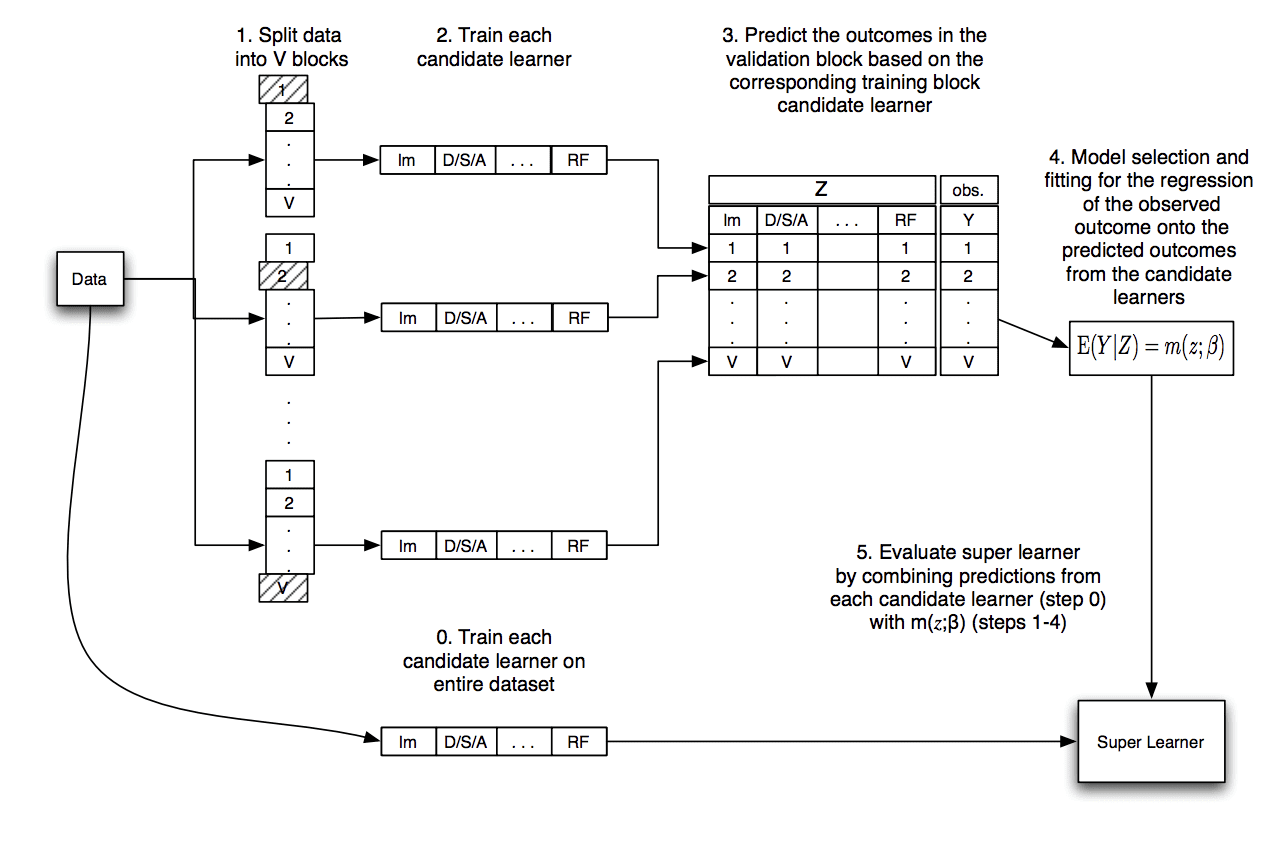
\includegraphics[width=\textwidth]{./Figures/sup-learn.jpg}
\end{figure}

\end{frame}

\begin{frame}[fragile]%{Super learner algorithm}

{%
\setlength{\interspacetitleruled}{0pt}%
\setlength{\algotitleheightrule}{0pt}%
\begin{algorithm}[H]
\KwIn{$\mathcal{D}=\set{(x_i,y_i)}_1^N$, $\mathcal{L}=\set{\phi_k(X)}_{k=1}^K$}
\ForEach{strong learner in $\mathcal{L}$}{%
	Fit $\phi_k$ on $\mathcal{D}$ $\Rightarrow$ $\hat{\phi}_k(\boldsymbol{X})$
	$\rightarrow$ $\hat{\mathcal{L}}=\set{\hat{\phi}_k}_{k=1}^K$\;
}
%Store the fitted library in $\hat{\mathcal{L}}=\set{\hat{\phi}_k(\boldsymbol{X})}_{k=1}^K$\;
\For{$\nu=1,2,\dots,V$}{%
	\ForEach{strong learner in $\mathcal{L}$}{%
		Fit $\phi_k$ on $T(\nu)$, predict $\hat{\phi}_{k,T(\nu)}(X_i\in V(\nu))$\;
	}
}
Stack output in an $N\times K$ matrix
%$Z=\Bigl\{\hat{\phi}_{k,T(\nu)}\bigl(X_{V(\nu)}\bigr),\,\nu=1,2,\dots,V,\,k=1,2,\dots,K\Bigr\}$\;
$Z=\bigl\{\hat{\phi}_{k,T(\nu)}\bigl(X_{V(\nu)}\bigr)\bigr\}$\;
Propose a family of weighted combinations\vspace{-1em}
\[
m(z\rvert\alpha)=\sum_{k=1}^K\alpha_k\hat{\phi}_{k,T(\nu)}\bigl(\boldsymbol{X}_{V(\nu)}\bigr)
\rightarrow
\hat{\alpha}=\argmin_\alpha\sum_{i=1}^NL(Y_i,m(z_i\rvert\alpha))
\vspace*{-1em}\]
of size $N$ s.t. $\alpha_k\geq0$, $\sum_k\alpha_k=1$ and minimizes $\sum_k\alpha_k\hat{\phi}_k$\;
Combine $\hat{\alpha}$ with the library $\hat{\mathcal{L}}$ $\rightarrow$ 
$\hat{\phi}_{\text{SL}}(\boldsymbol{X})=\sum_{k=1}^K\hat{\alpha}_k\hat{\phi}_k(\boldsymbol{X})$\;
\KwOut{$\hat{\phi}_{\text{SL}}$}
\end{algorithm}}

\end{frame}


\end{document}
